\documentclass[a4paper]{article}

%% Language and font encodings
\usepackage[english]{babel}
\usepackage[utf8x]{inputenc}
\usepackage[T1]{fontenc}


%% Sets page size and margins
\usepackage[a4paper,top=3cm,bottom=2cm,left=3cm,right=3cm,marginparwidth=1.75cm]{geometry}
\usepackage{amsmath}
\usepackage{amsthm}

\newtheorem{theorem}{Theorem}
\newtheorem{lemma}[theorem]{Lemma}

\usepackage{graphicx}
\usepackage{qtree}

\begin{document}
\section*{Implicit navigation in vEB layout}
Consider $N = 2h − 1$ keys where $h$ is a power of 2,
and the implicit cache-oblivious vEB layout of their corresponding complete binary
tree, where the keys are suitably permuted and stored in an array of length N without
using pointers (as it happens in the classical implicit binary heap but the rule here
is different). The root is in the first position of the array. Find a rule that, given the
position of the current node, it is possible to locate in the array the positions of its
left and right children. Discuss how to apply this layout to obtain (a) a static binary
search tree and (b) a heap data structure, discussing the cache complexity
\\
\\
\textbf{SOLUTION}
\subsection*{Assumptions}
Suppose you have a binary vEB tree $T$ stored in an array \texttt{T[]} in external memory, as seen in class, ordered as in the tree's induced "fractal" numbering, starting from 0:

\Tree
[.0 
	[.1
		[.3 4 5 ]
		[.6 7 8 ]
	]
	[.2
		[.9 10 11 ]
		[.12 13 14 ]
	]
]
\\
This is the same order in which elements are stored in \texttt{T[]}


Let the tree be complete and let its height, \texttt{H}, be a power of two. Also suppose you can store \texttt{H} locally.
\\
\begin{tiny}N.B. In the code that follows, all division signs (\texttt{/}) represent integer division (div).\end{tiny}

\subsection*{ZoomSequence}
The following function generates a sequence $zs$ of indexes of \emph{nested} subtrees of $T$ that uniquely identifies the position of node \texttt{target} in both $T$ and \texttt{T[]}.

Starting from $T$, the decomposition will split a generic binary vEB tree $A$ of height $h$ into a \emph{top tree} of index $0$ and height $\frac{h}{2}$ and $2^\frac{h}{2}$ \emph{bottom trees} (two per leaf of the top tree) of indexes 1\dots $2^\frac{h}{2}$ and again height $2^\frac{h}{2}$.

An element $zs_i$ will thus correspond to the index of a subtree of height $2^\frac{H}{2^{i+1}}$, nested into the subtree identified by $zs_{i-1}$ (or $T$ for $zs_0$).

Note that the sequence $zs$ contains exactly $log_2(H)$ entries.
\begin{verbatim}
ZoomSequence(target, H)
  let zs = Sequence.Empty; /* empty ordered list, first element will have index 0 */
  let h = H, i = target, blocksize = 0;
  while (h > 1)
    blocksize = 2^(h/2) -1;
    zs.Enqueue(i/blocksize);
    i = i mod blocksize;
    h = h/2;
  end
  return zs;
end
\end{verbatim}

Note that this requires no accesses to the tree, generating no cachefaults.


\subsection*{GetChildren}
The following (absolutely horrific...) function returns the \emph{tree node} indexes of the left and right children of tree node \texttt{i}. These can be fed to \texttt{GetElement} to obtain the contents of the actual nodes.

The basic idea is to traverse $zs$ looking for the largest $j$ such that $zs_j = 0$, which identifies the biggest vEB subtree that i is a leaf of (it is $T$ if there is no such $j$, which means i has no children). Then it is a matter of going up one level from that, and moving ahead by an appropriate amount of subtrees of height $\frac{H}{2^{j+1}}$.
\begin{verbatim}
GetChildren(i)
  if (i mod 3 = 0) then /* subtrees of height 2 are stored consecutively */
    return <i+1, i+2>; /* note that such children nodes necessarily exist
      because T is a complete tree */
  end
  let zs = ZoomSequence(i, H);
  let idx0 = zs.FirstIndexOf(0);  /* index of the first occurrence of 0 in zs
    or -1 if no such element exists */
  if (idx0 = -1) then /* i is a leaf of T, so it has no children */
    return <-1, -1>
  end
  /* from here on out we're sure we're not a leaf of T itself */
  let h = H, blocksize = 0;
  let k = H/2^(idx0+1); /* height of the biggest tree i is a leaf of */
  let off = 0; /* will be the index of the root of the tree immediately
    encompassing the biggest tree i is a leaf of */
  for i = 0 to idx0-1 do
    blocksize = 2^(h/2)-1;
    off = off + zs.Get(i)*blocksize;
    h = h/2;
  end
  h = H;
  let leafidx = 0; /* leafidx will be s.t. i is the leafidx-th leaf
    of the tree of height k, starting from 0 */
  for i = idx0+1 to zs.Length do /* stuff following last zero element in zs */
    leafidx = (zs.Get(i)-1);
    h = h/2;
  end
  let left = off + (2^k -1)*(2*leafidx +1); /* 2 children per leaf of top tree
    +1 because of top tree */
  let right = off + (2^k -1)*(2*leafidx +2); /* +2 because of top tree and left child */
  return <left, right>;
end
\end{verbatim}
Again, the function never accessed the tree itself, generating no cachefaults.

\subsection*{Binary Search Tree}
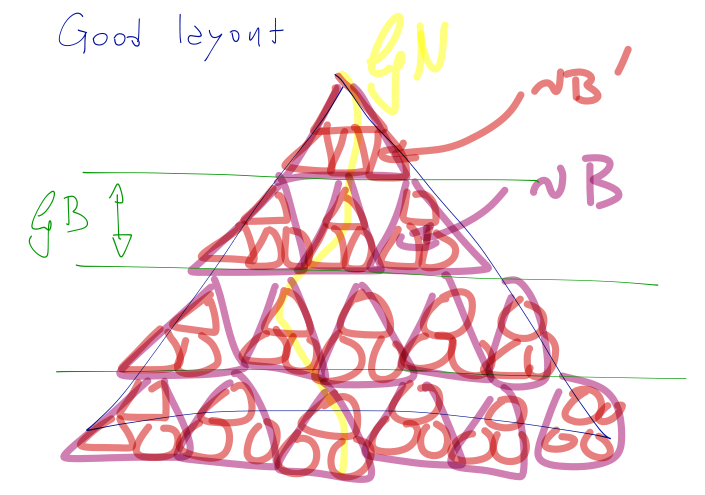
\includegraphics[scale = 0.65]{pic}

As is quite evident from Professor Grossi's very excellent picture, given any block size $B$ (which we can reasonably assume to be a power of two), a block will be able to hold a subtree of height $log_2(B)$.

For a binary vEB tree $T$ made up of $N$ nodes, a single lookup will traverse $H = log_2(N)$ nodes. Such nodes residing into blocked memory, we will observe a total of $$O\bigg(\frac{log_2(N)}{log_2(B)}\bigg) = O(log_B(N))$$ cachefaults.

\end{document}
